\documentclass{standalone}
\usepackage{tikz}
\usetikzlibrary{patterns}
\usetikzlibrary{positioning}
\usetikzlibrary{patterns, positioning}
\usetikzlibrary{shapes.misc}
\usepackage[outline]{contour}
\contourlength{1.5pt} 
\usepackage[sfdefault]{ClearSans}

\begin{document}
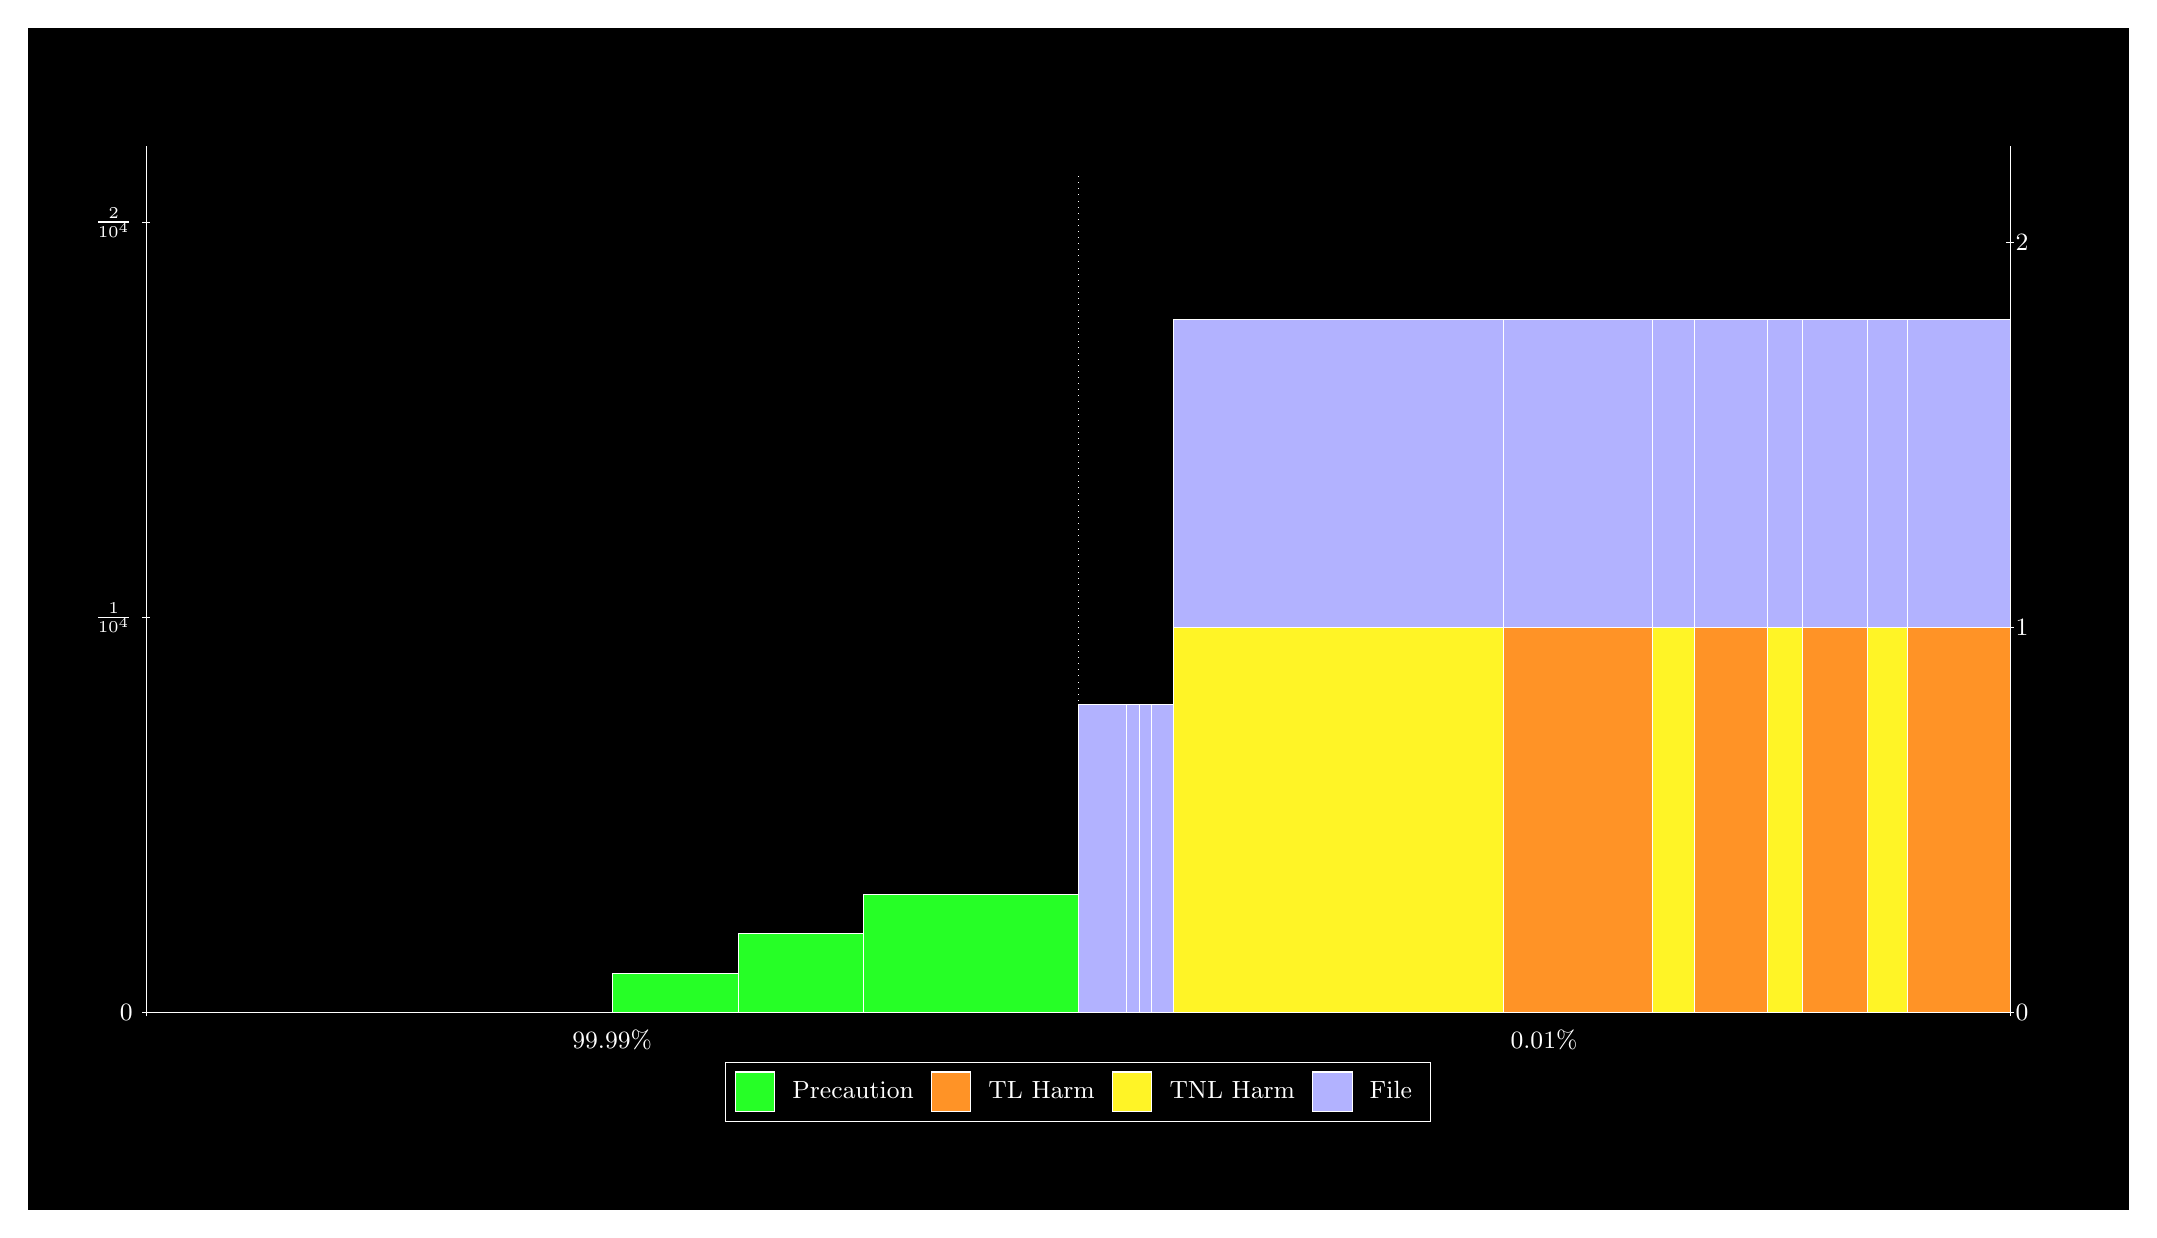
\begin{tikzpicture}
\draw[fill=black] (0,0) rectangle (26.667,15);
\draw[fill=green!85,draw=white,very thin] (7.4166,2.5) rectangle (9.0126,3.0017);
\draw[fill=green!85,draw=white,very thin] (9.0126,2.5) rectangle (10.611,3.5035);
\draw[fill=green!85,draw=white,very thin] (10.611,2.5) rectangle (13.333,4.0052);
\draw[fill=blue!30,draw=white,very thin] (13.333,2.5) rectangle (13.94,6.411);
\draw[fill=green!85,draw=white,very thin] (13.94,2.5) rectangle (14.104,2.5);
\draw[fill=blue!30,draw=white,very thin] (13.94,2.5) rectangle (14.104,6.4111);
\draw[fill=green!85,draw=white,very thin] (14.104,2.5) rectangle (14.268,2.5001);
\draw[fill=blue!30,draw=white,very thin] (14.104,2.5001) rectangle (14.268,6.4111);
\draw[fill=green!85,draw=white,very thin] (14.268,2.5) rectangle (14.548,2.5001);
\draw[fill=blue!30,draw=white,very thin] (14.268,2.5001) rectangle (14.548,6.4112);
\draw[fill=yellow!85,draw=white,very thin] (14.548,2.5) rectangle (18.728,7.3888);
\draw[fill=blue!30,draw=white,very thin] (14.548,7.3888) rectangle (18.728,11.3);
\draw[fill=orange!85,draw=white,very thin] (18.728,2.5) rectangle (20.62,7.3888);
\draw[fill=blue!30,draw=white,very thin] (18.728,7.3888) rectangle (20.62,11.3);
\draw[fill=green!85,draw=white,very thin] (20.62,2.5) rectangle (21.163,2.5);
\draw[fill=yellow!85,draw=white,very thin] (20.62,2.5) rectangle (21.163,7.3889);
\draw[fill=blue!30,draw=white,very thin] (20.62,7.3889) rectangle (21.163,11.3);
\draw[fill=green!85,draw=white,very thin] (21.163,2.5) rectangle (22.081,2.5);
\draw[fill=orange!85,draw=white,very thin] (21.163,2.5) rectangle (22.081,7.3889);
\draw[fill=blue!30,draw=white,very thin] (21.163,7.3889) rectangle (22.081,11.3);
\draw[fill=green!85,draw=white,very thin] (22.081,2.5) rectangle (22.526,2.5001);
\draw[fill=yellow!85,draw=white,very thin] (22.081,2.5001) rectangle (22.526,7.3889);
\draw[fill=blue!30,draw=white,very thin] (22.081,7.3889) rectangle (22.526,11.3);
\draw[fill=green!85,draw=white,very thin] (22.526,2.5) rectangle (23.35,2.5001);
\draw[fill=orange!85,draw=white,very thin] (22.526,2.5001) rectangle (23.35,7.3889);
\draw[fill=blue!30,draw=white,very thin] (22.526,7.3889) rectangle (23.35,11.3);
\draw[fill=green!85,draw=white,very thin] (23.35,2.5) rectangle (23.867,2.5001);
\draw[fill=yellow!85,draw=white,very thin] (23.35,2.5001) rectangle (23.867,7.389);
\draw[fill=blue!30,draw=white,very thin] (23.35,7.389) rectangle (23.867,11.3);
\draw[fill=green!85,draw=white,very thin] (23.867,2.5) rectangle (25.167,2.5001);
\draw[fill=orange!85,draw=white,very thin] (23.867,2.5001) rectangle (25.167,7.389);
\draw[fill=blue!30,draw=white,very thin] (23.867,7.389) rectangle (25.167,11.3);
\draw[white,very thin] (1.5,2.5) -- (1.5,13.5);
\draw[white,very thin] (1.45,2.5) -- (1.55,2.5);
\node[font=\small,text=white, anchor=east] at (1.45, 2.5) {0};
\draw[white,very thin] (1.45,7.5173) -- (1.55,7.5173);
\node[font=\small,text=white, anchor=east] at (1.45, 7.5173) {$\frac{1}{10^{4}}$};
\draw[white,very thin] (1.45,12.535) -- (1.55,12.535);
\node[font=\small,text=white, anchor=east] at (1.45, 12.535) {$\frac{2}{10^{4}}$};

\draw[white,dotted,very thin] (13.333,2.83) -- (13.333,13.17);
\draw[white,very thin] (25.167,2.5) -- (25.167,13.5);
\draw[white,very thin] (25.117,2.5) -- (25.217,2.5);
\node[font=\small,text=white, anchor=west] at (25.117, 2.5) {0};
\draw[white,very thin] (25.117,7.3888) -- (25.217,7.3888);
\node[font=\small,text=white, anchor=west] at (25.117, 7.3888) {1};
\draw[white,very thin] (25.117,12.278) -- (25.217,12.278);
\node[font=\small,text=white, anchor=west] at (25.117, 12.278) {2};

\draw[white,very thin] (1.5,2.5) -- (25.167,2.5);
\draw[white,very thin] (1.5,2.45) -- (1.5,2.55);
\node[font=\small,text=white, anchor=north] at (1.5, 2.45) {};
\draw[white,very thin] (25.167,2.45) -- (25.167,2.55);
\node[font=\small,text=white, anchor=north] at (25.167, 2.45) {};

\node[font=\small,text=white,anchor=south] at (7.4167, 1.9) {99.99\%};
\node[font=\small,text=white,anchor=south] at (19.25, 1.9) {0.01\%};
\draw (13.3333,2.5) node (B) {};
\begin{scope}[align=center]
\matrix[scale=0.5,draw=white,below=0.5cm of B,nodes={draw},column sep=0.1cm]{
\node[rectangle,draw,minimum width=0.5cm,minimum height=0.5cm,fill=green!85]{}; & \node[draw=none,font=\small,text=white]{Precaution}; &
\node[rectangle,draw,minimum width=0.5cm,minimum height=0.5cm,fill=orange!85]{}; & \node[draw=none,font=\small,text=white]{TL Harm}; &
\node[rectangle,draw,minimum width=0.5cm,minimum height=0.5cm,fill=yellow!85]{}; & \node[draw=none,font=\small,text=white]{TNL Harm}; &
\node[rectangle,draw,minimum width=0.5cm,minimum height=0.5cm,fill=blue!30]{}; & \node[draw=none,font=\small,text=white]{File}; \\\\
};\end{scope}

\end{tikzpicture}
\end{document}